\pdfbookmark[0]{\contentsname}{toc}
\tableofcontents*
\cleardoublepage

\chapter{Lista de Exercícios 3}

\section{Questão 1.1 - Forneça o valor calculado da pressão acústica.}
Para o cálculo da pressão acústica utilizou-se a seguinte sequência de processamento:
\begin{enumerate}
	\item Os dados de velocidades das matrizes Ux, Uy e Uz foram importados nas variáveis
``velocidades.vel\_x'', ``velocidades.vel\_y'' e ``velocidades.vel\_z'' respectivamente;
	\item Valores físicos para densidade inicial, comprimento elementar e posição do ouvinte no espaço foram definidos;
	\item A função ``calcular\_pressao()'' foi chamada para o calculo da pressao;
	\item Dentro da função ``calcular\_pressao()'' foram dados os seguintes processos:
	\begin{enumerate} 
		\item Foi calculado o valor de \begin{math}vivj\end{math} através soma de todas as velocidades elevadas ao quadrado (simplificação do Tensor de Lighthill);
		\item \begin{math}vivj\end{math} foi multiplicado pela densidade inicial;
		\item Foi construída uma matriz unitária de dimensões 100 X 95 X 100 no intuito de preenchê-la com o escalar calculado anteriormente;
		\item Foi calculado a subtração da posição do observador por cada ponto da região de turbulência;
		\item Derivou-se, para cada direção, 2 vezes, objetivando calcular o laplaciano do Tensor de Lighthill;
		\item Integrou-se o resultado através de integral de volume com o método numérico trapeziodal.
	\end{enumerate}
\end{enumerate}

Segue o código do $script$ principal:
	\begin{lstlisting}
	clear('all');
	close all;

	% Lista de Exercicios 3

	disp('Questao 1.1 ----------------------');
	velocidades = open('velocidades.mat');
	velocidades_x = velocidades.vel_x(:,:,1);
	velocidades_y = velocidades.vel_y(:,:,1);
	rho = 1.2; % kg/m^3
	delta_x = 0.003; % m
	posicao_ouvinte = [15 15 15]; % m

	pressao_acustica = calcular_pressao(rho, delta_x, ...
	velocidades.vel_x, velocidades.vel_y, ...
	posicao_ouvinte);

	valor_referencia = 2*10^-5;
	nivel_pressao_sonora_dB = 20*log10((pressao_acustica ...
	+valor_referencia)/valor_referencia);
	\end{lstlisting}

	Segue a função ``calcular\_pressao()'':
	\begin{lstlisting}
	function pressao_acustica = calcular_pressao ... 
	(rho, delta_x, velocidades_x, ...
	velocidades_y, posicao_ouvinte)

	% Calculando o vi*vj
	vi_vj = (sum(sum(sum(velocidades_x.^2))) + ... 
	sum(sum(sum(velocidades_y.^2))));
	% Calculando o rho*vi*vj
	rho_vi_vj = rho*vi_vj;

	% Preenchendo a matriz pelo escalar rho_vi_vj
	matriz_tensor_lighthill = velocidades_x;
	matriz_tensor_lighthill(:) = 1;
	matriz_tensor_lighthill = matriz_tensor_lighthill*rho_vi_vj;

	% Calculando a distancia |x - y|
	tamanhos = size(velocidades_x);
	for x = 1:tamanhos(1)
		for y = 1:tamanhos(2)
			for z = 1:tamanhos(3)
				posicao_x = posicao_ouvinte(1) - x*0.003;
				posicao_y = posicao_ouvinte(2) - y*0.003;
				posicao_z = posicao_ouvinte(3) - z*0.003;
				distancia = sqrt(posicao_x^2 + ... 
				posicao_y^2 + posicao_z^2);
				A = matriz_tensor_lighthill(x, y, z);
				B =  4*pi*distancia;
				B = 1/B;
				matriz_tensor_lighthill(x, y, z) = A*B;
			end
		end
	end

	% Calculando o laplaciano para depois integrar
	diferenciado_x_tensor_lighthill = ... 
	diff(matriz_tensor_lighthill, 2, 1);
	diferenciado_x_tensor_lighthill = ... 
	diferenciado_x_tensor_lighthill;
	diferenciado_xy_tensor_lighthill = ... 
	diff(diferenciado_x_tensor_lighthill, 2, 2);
	diferenciado_xy_tensor_lighthill = ... 
	diferenciado_xy_tensor_lighthill;
	diferenciado_xyz_tensor_lighthill = ... 
	diff(diferenciado_xy_tensor_lighthill, 2, 3);
	laplaciano_tensor_lighthill = diferenciado_xyz_tensor_lighthill;

	% Calculando a pressao final
	pressao_acustica_x = trapz(laplaciano_tensor_lighthill,1);
	pressao_acustica_xy = trapz(pressao_acustica_x,2);
	pressao_acustica = trapz(pressao_acustica_xy,3);
	\end{lstlisting}

	Dos resultados tem-se:
	\begin{itemize}
		\item Valor de Pressão Acústica: 6.05360e-09 N/m²;
		\item Valor de Nível de Pressao Sonora: 0.0026286 dB.	
	\end{itemize}
	

	\section{Questão 1.2 - Plote os mapas de superfície e encontre a dimensão característica $l$.}
	Segue o código da questão:
	\begin{lstlisting}
	disp('Questao 1.2 ----------------------');
	% Plotando mapa de superficie de velocidade absoluta
	velocidades_absolutas = sqrt(velocidades_x.^2 + ...
	velocidades_y.^2);
	[x,y] = meshgrid([0:99]*0.003);
	x = x(:, 1:95);
	y = y(:, 1:95);
	figure;
	surf(velocidades_absolutas);
	title('Grafico de Velocidades Absolutas');
	xlabel('x');
	ylabel('y');
	zlabel('velocidade absoluta [m/s]');
	vorticidade = curl(velocidades_x, velocidades_y);
	figure;
	surf(x, y, vorticidade);
	title('Grafico de Velocidades Vorticiais');
	ylabel('y');
	xlabel('x');
	zlabel('velocidade vorticial [rad/s]');
	\end{lstlisting}

	Segue o gráfico de superfície da velocidade absoluta:
	\begin{figure}[h]
	\centering
		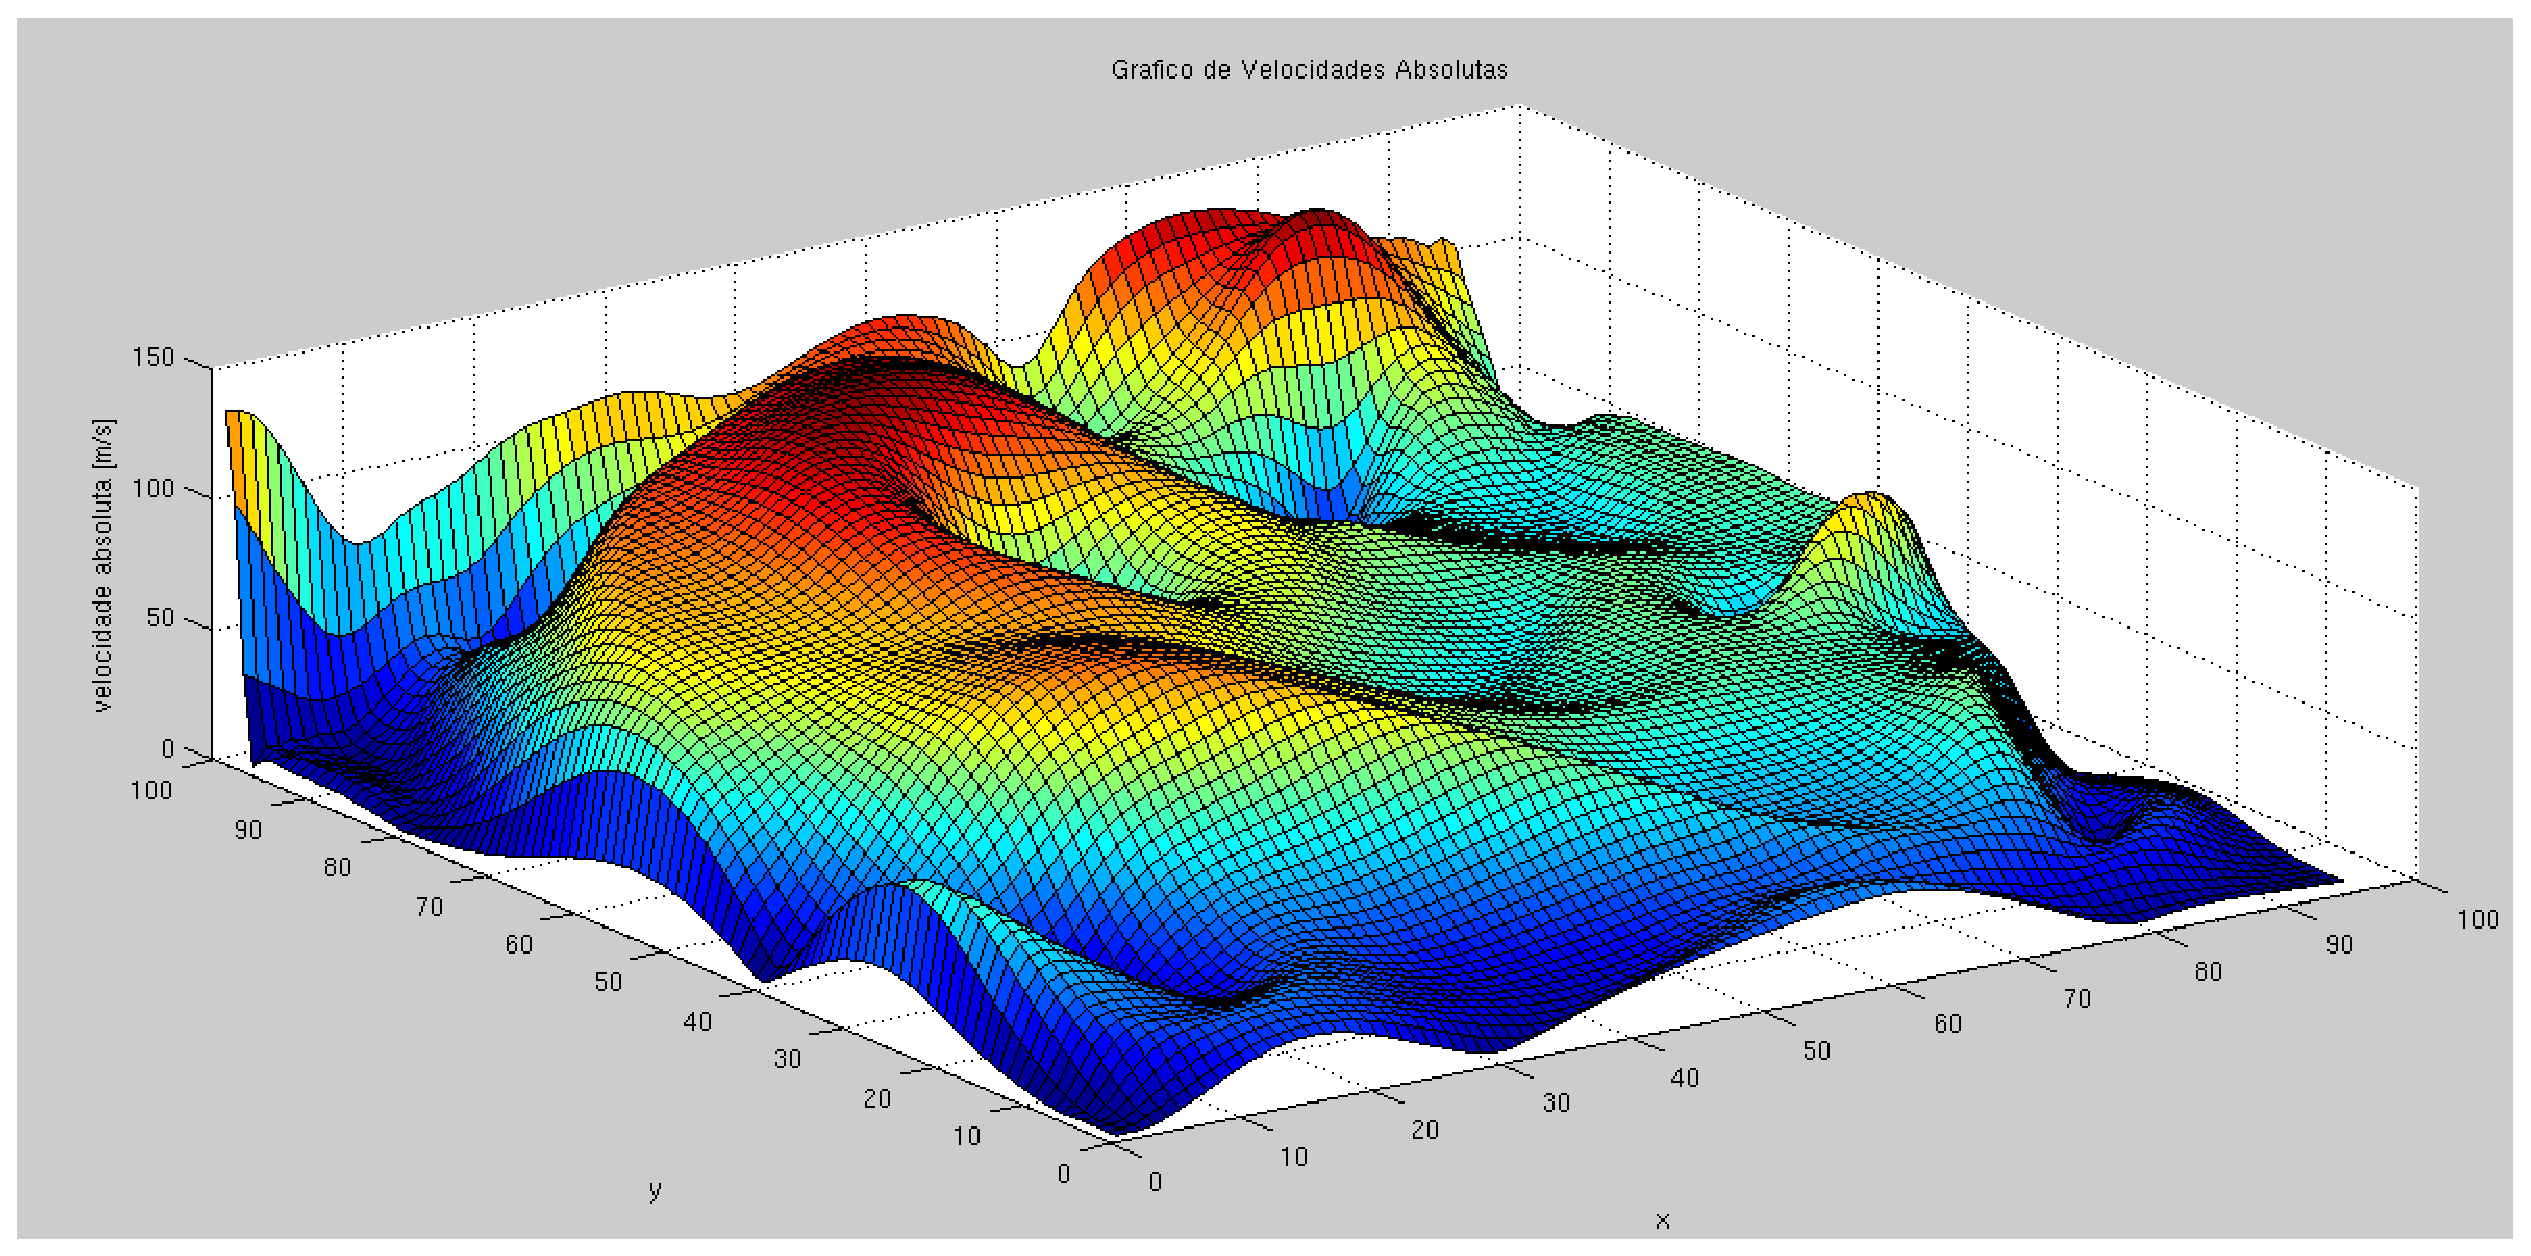
\includegraphics[keepaspectratio=true,scale=0.4]{figuras/velocidade_absoluta.eps}
	\end{figure}

	Segue o gráfico de superfície da vorticidade:
	\begin{figure}[h]
	\centering
		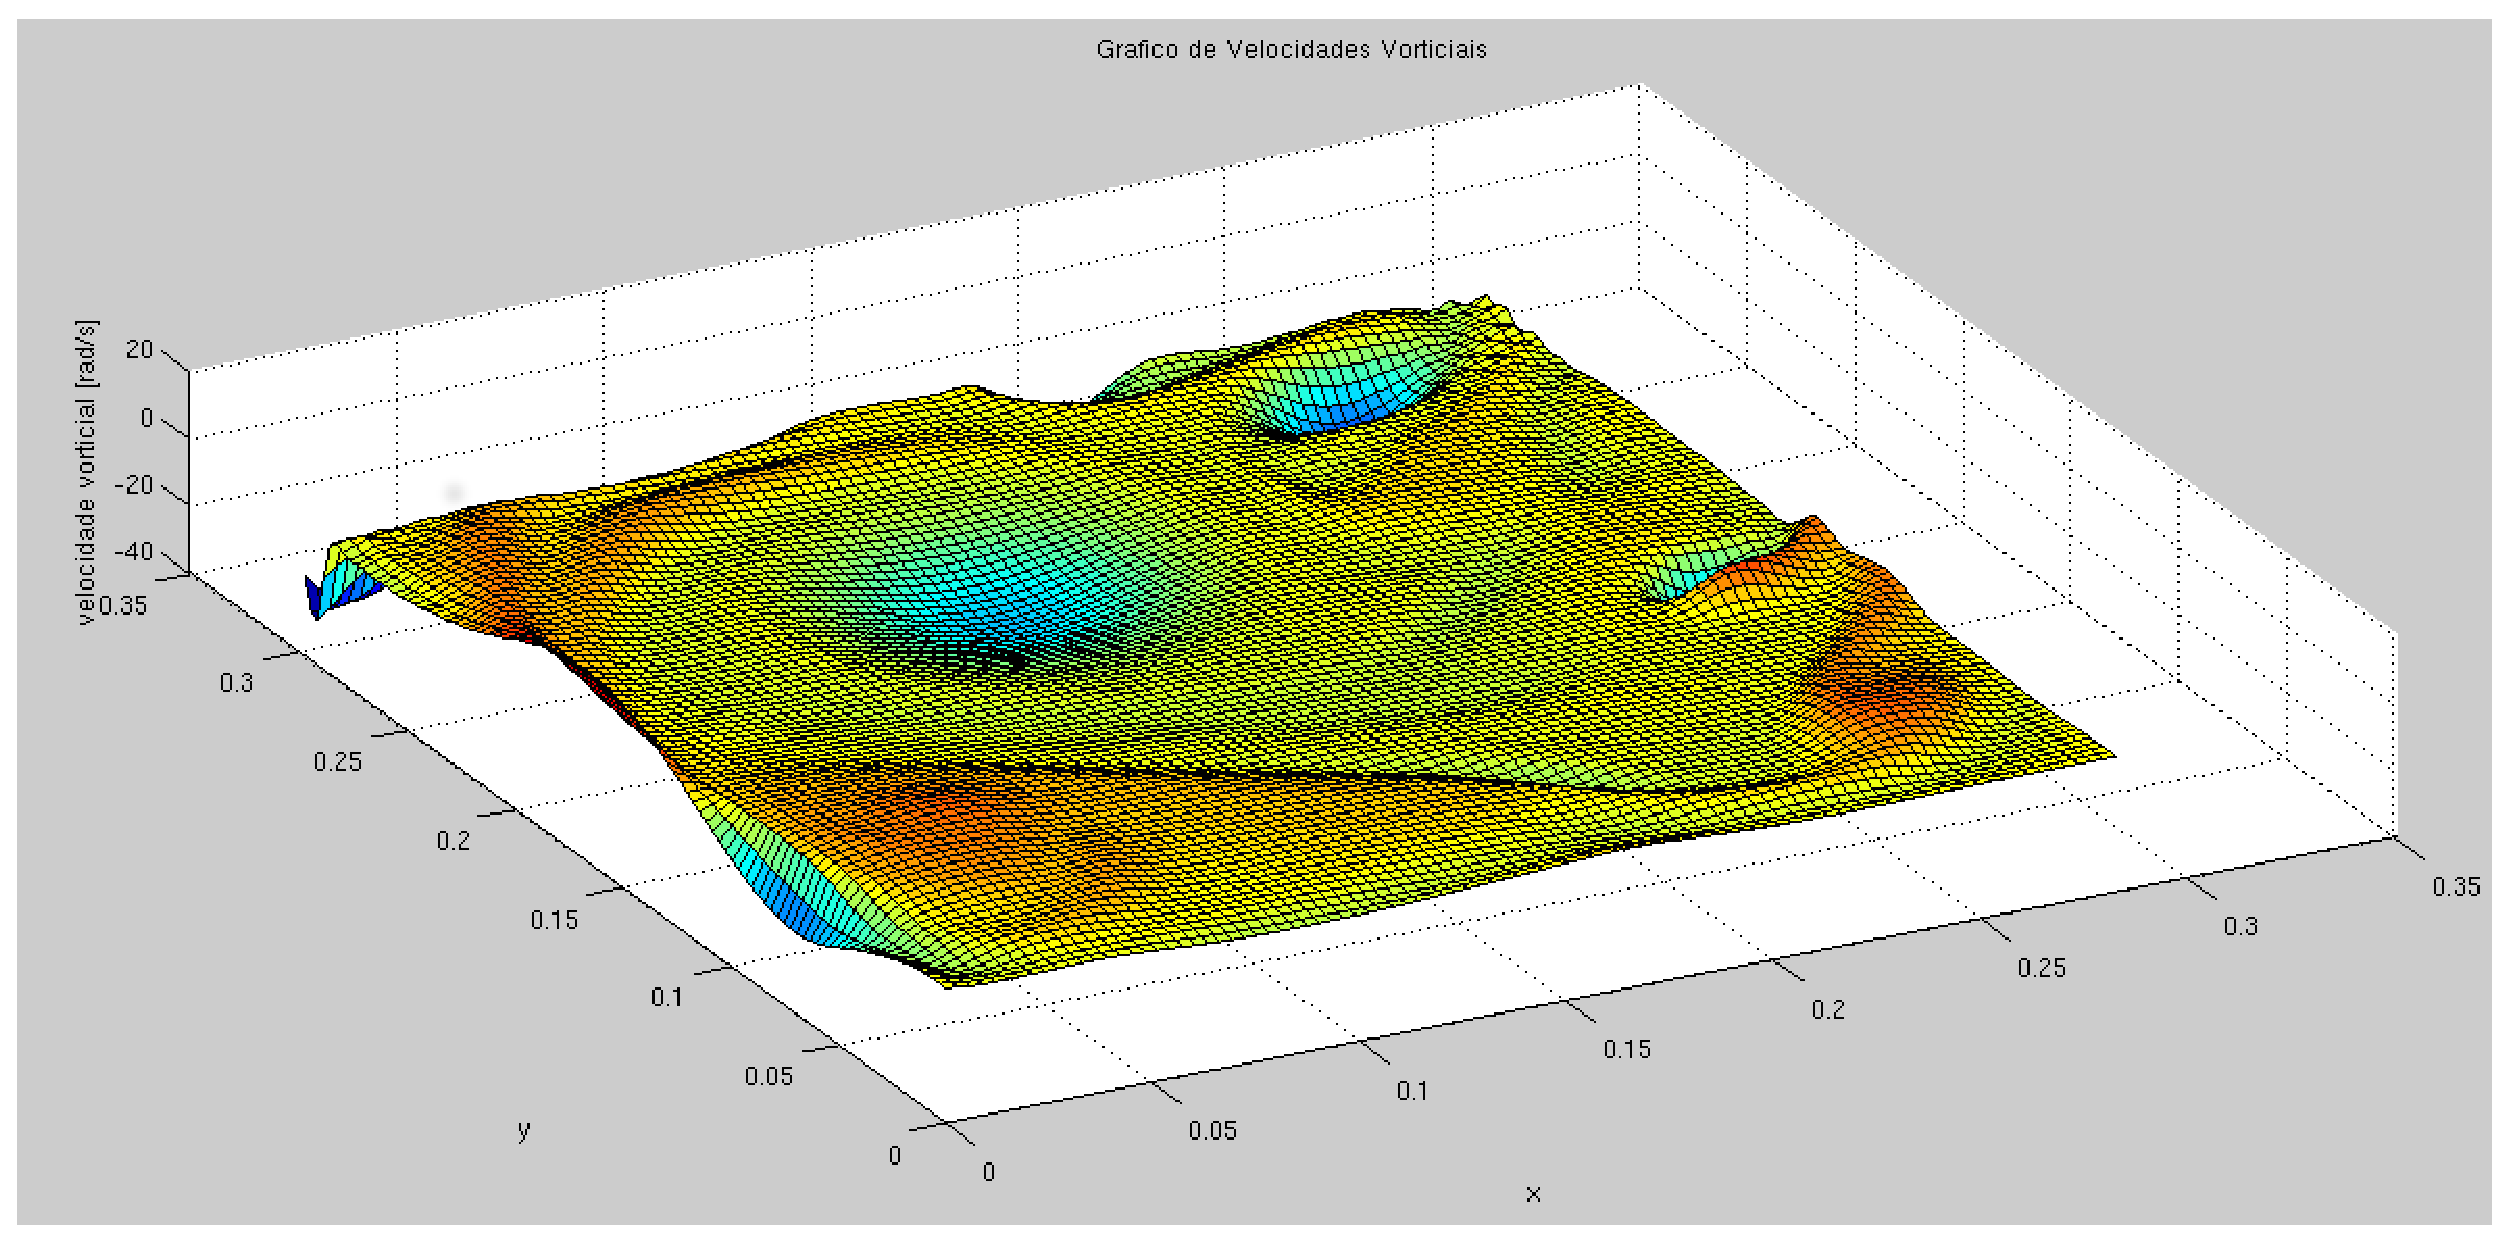
\includegraphics[keepaspectratio=true,scale=0.4]{figuras/vorticidade.eps}
	\end{figure}


	Dado os 2 gráficos o valor aproximado da dimensão característica é de 0.0630 metros ou 63 mm, pois a turbulência possui um centro definido com esse diâmetro característico.

	\section{Questão 3 - A partir da Eq(1) e da Eq(2) plote gráficos e compare-os. Os resultados coincidem? Justifique a sua resposta de maneira crítica.}

	Segue o código em questão:
	\begin{lstlisting}
	clear('all');
	close all;

	% Lista de Exercicios 3

	disp('Questao 1.3 ----------------------');
	dimensao_caracteristica_l = 0.063; % m
	distancia = sqrt(sum(posicao_ouvinte.^2)); % m 
	c0 = 340; % m/s 
	velocidade_inicial = ((pressao_acustica* ... 
	(distancia)*c0^2)/(dimensao_caracteristica_l*rho))^(1/4);
	% Plotando grafico de pressao por ...
	% velocidades atraves da equacao 1
	pressao_velocidades_1(1:10) = 0;
	pressao_velocidades_2(1:10) = 0;
	velocidades_media_x = velocidades.vel_x;
	tamanhos = size(velocidades.vel_x);
	velocidade_media_x = (sum(sum(sum(velocidades_x)))) ... 
	/tamanhos(1)*tamanhos(2)*tamanhos(3);
	velocidades_media_x(:) = 1;
	velocidades_media_x = velocidades_media_x*velocidade_media_x;
	velocidades_media_y = velocidades.vel_y;
	tamanhos = size(velocidades.vel_y);
	velocidade_media_y = (sum(sum(sum(velocidades_y)))) ... 
	/tamanhos(1)*tamanhos(2)*tamanhos(3);
	velocidades_media_y(:) = 1;
	velocidades_media_y = velocidades_media_y* ... 
	velocidade_media_y;
	for divisao = 1:10
		velocidade_divisao = 10^divisao;
		pressao_velocidades_1(divisao) = calcular_pressao(rho, ...
		delta_x, velocidades_media_x/velocidade_divisao ...
		, velocidades_media_y/velocidade_divisao, posicao_ouvinte);
		velocidade = velocidade_inicial/velocidade_divisao;
		pressao_velocidades_2(divisao) = (dimensao_caracteristica_l ... 
		/distancia)*(rho*velocidade^4)/c0^2;
	end	
	figure;
	loglog(pressao_velocidades_1);
	hold on;
	loglog(pressao_velocidades_2, 'r');
	title('Grafico Pressao Sonora em Relacao a Velocidade Absoluta');
	ylabel('pressao acustica');
	xlabel('velocidade');
	legend('Equacao de Lighthill', 'Aproximacao da Oitava Potencia');
	\end{lstlisting}

 Gráfico resultante da questão:
 \begin{figure}[h]
	\centering
		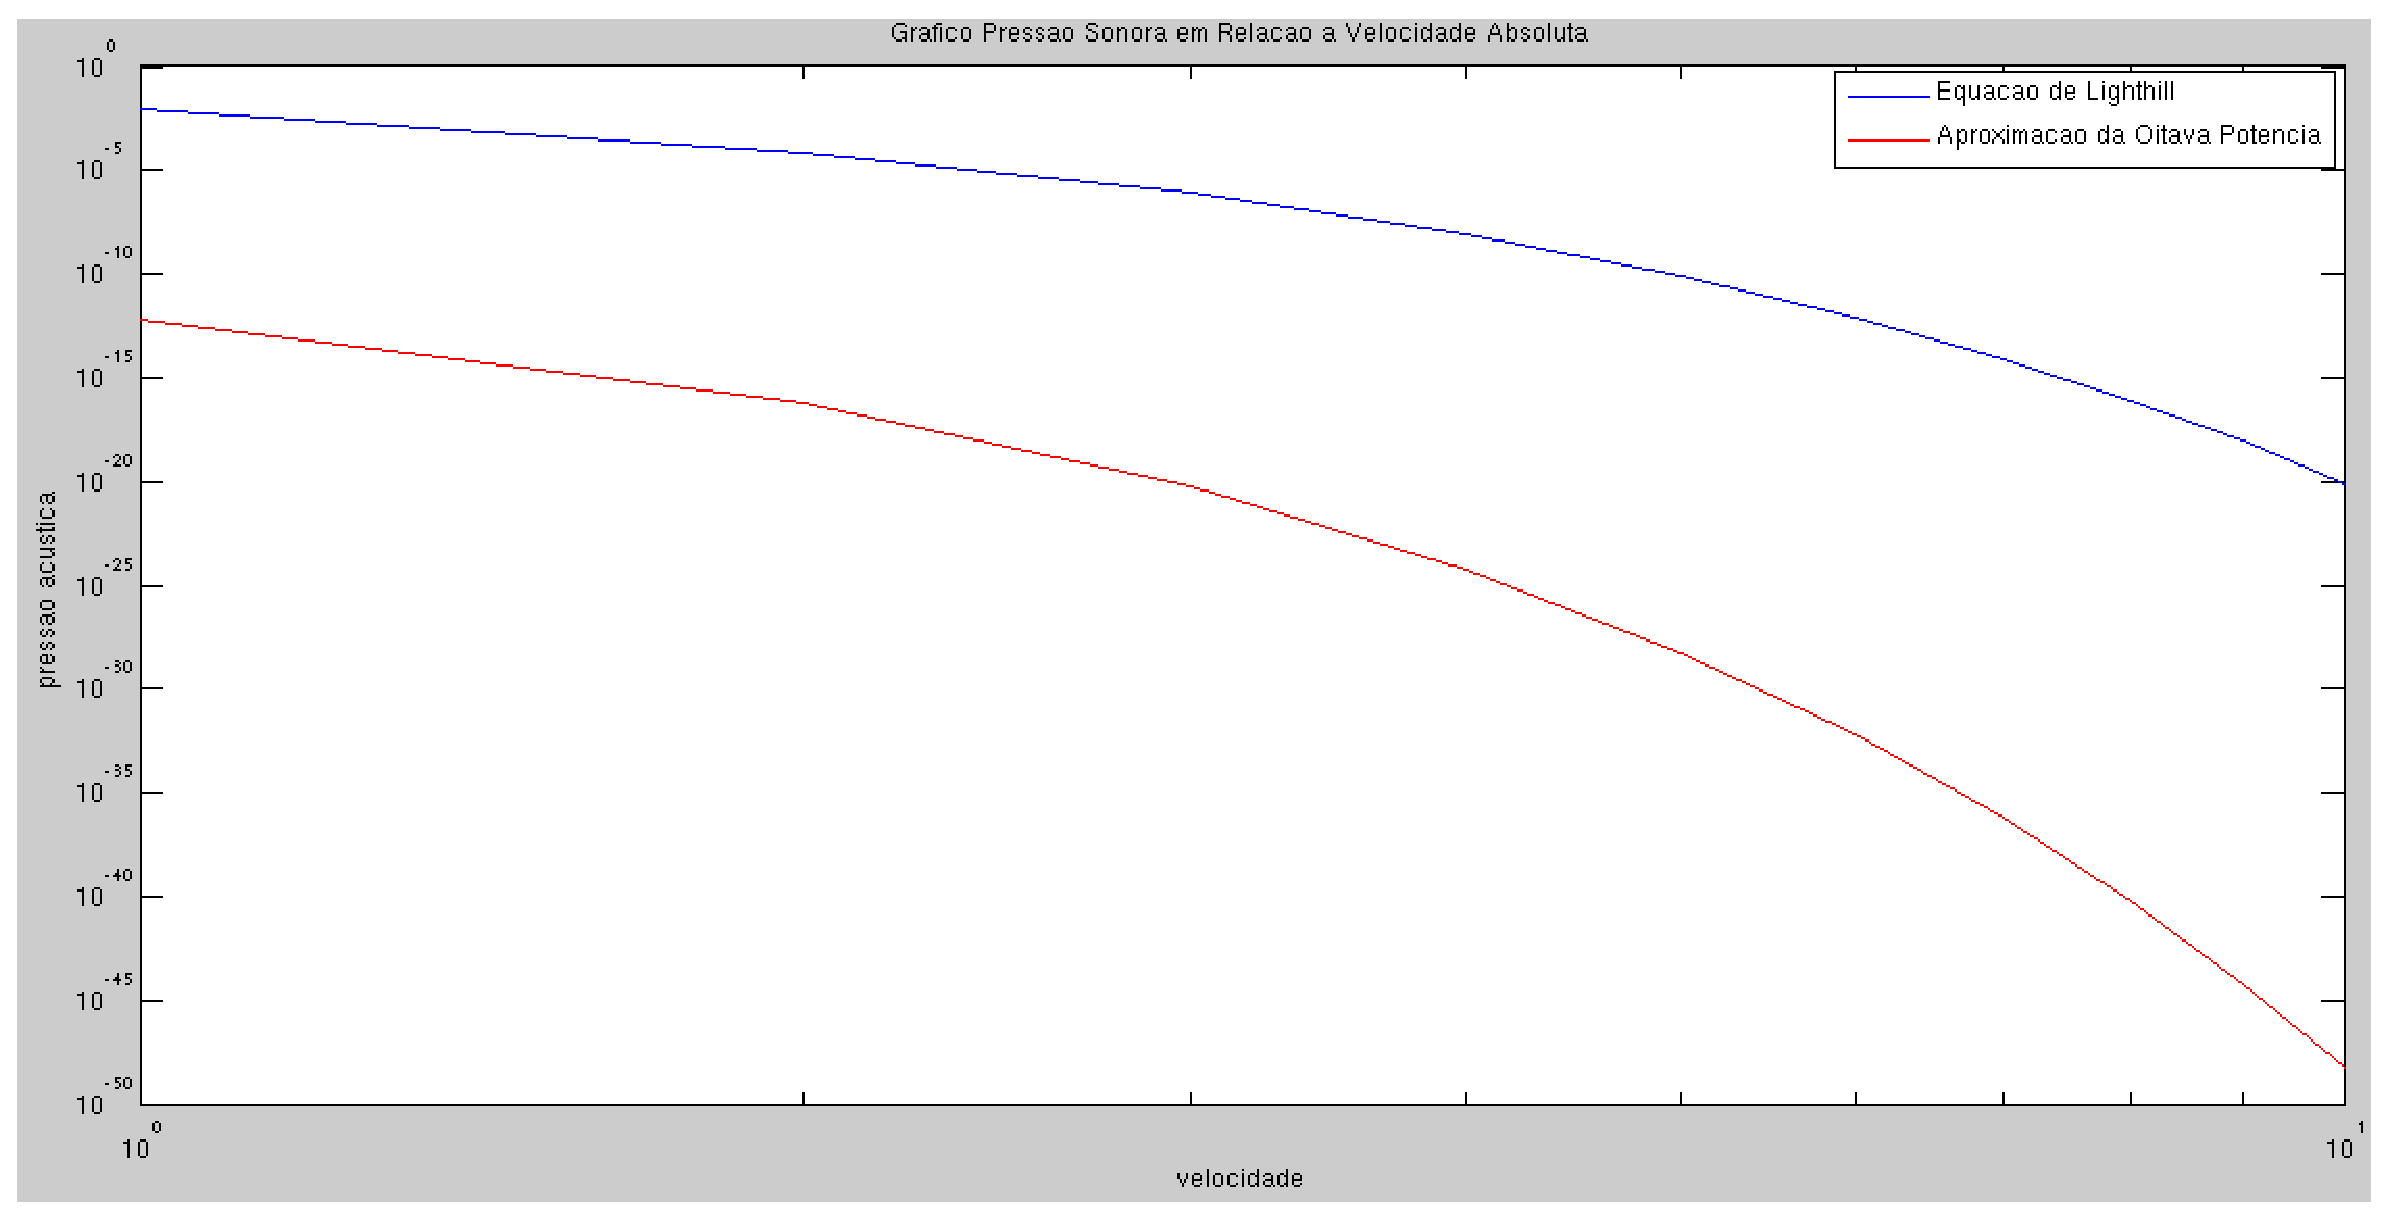
\includegraphics[keepaspectratio=true,scale=0.4]{figuras/pressao_velocidade.eps}
	\end{figure}			

 Os dois gráficos possuem comportamentos similares visto que a pressão sonora decai exponencialmente ao longo
 da variação de velocidades. Esse fato ocorre pois nas duas equações se considera que o som é gerado a partir 
 de somas compactas oriundas de fontes sonoras, independentes,
 que possuem o volume definido por V0/l³, dado que l é a dimensão característica de cada vórtice.
 Dado esse contexto, na expansão em campo distante o termo de retardamento se aproxima de 0 pois é considerado
 que a análise dos vórtices é feita na origem do sistema, desconsiderando assim o efeito do retardamento. Nesse caso
 a integral da solução de Green em campo distante se delimita em $\rho$v²l³.

 \section{Questão 2.1 - Quais os procedimentos para calcular a potência sonora instantânea?}

 O cálculo para o corolário de Howe seguirá os seguintes passos:
 \begin{enumerate}
 		\item Aplicar o operador $curl()$ na matriz de velocidades $V$. $Curl$: operador que descreve a rotação de um campo de velocidades vetorial tridimensional;
 		\item Realizar a multiplicação vetorial entre $\omega$(componente rotacional da velocidade) e $V$ (velocidade);
 		\item Aplicar a multiplicação do escalar velocidade de partícula ($v'$) pelo produto vetorial de $\omega$ x $V$;
 		\item Realizar a integração do volume do vórtice por meio da função de integração numérica trapezoidal;
 		\item Multiplicar a solução desta integral por $-\rho$.
 \end{enumerate}

 \section{Questão 2.2 - Determine a potência instantânea considerando que $v'$ = [0, 0, 35] m/s.}

 Segue o código do mesmo:
 \begin{lstlisting}
% Declarando v_linha
v_linha = [0 0 35];
% Calculando a vortidade
vorticidade = curl(velocidades.vel_x(:,:,1), ...
velocidades.vel_y(:,:,1));
% Calculando a vortidade media para redistribuir numa tridimensional
vorticidade_media = mean(mean(mean(vorticidade)));
% Preenchendo a matriz de vorticidades
matriz_vorticidade = velocidades.vel_x;
matriz_vorticidade(:) = 1;
vorticidade = matriz_vorticidade*vorticidade_media;
% Tamanhos totais
tamanhos = size(vorticidade);
% Construindo a matriz w_v_vlinha
matriz_w_v_vlinha = velocidades.vel_x(:,:,1);
% Calculando ponto a ponto o produto vetorial
for x = 1:tamanhos(1)
	for y = 1:tamanhos(2)
		for z = 1:tamanhos(3)
			termo_1 = [vorticidade(x,y,z) ...
			vorticidade(x,y,z) ... 
			vorticidade(x,y,z)];
			termo_2 = [velocidades.vel_x(x,y,z) ...
			velocidades.vel_y(x,y,z) ...
			velocidades.vel_z(x,y,z)];
			% Produto vetorial da vorticidade com as velocidades
			produto_vetorial = cross(termo_1, termo_2);
			% Produto escalar do produto vetorial com o v_linha
			matriz_w_v_vlinha(x,y,z) = sum(produto_vetorial.*v_linha);
		end
	end
end

% Integrando a matriz oriunda de w, v e v'
integracao_x_matriz_w_v_vlinha = trapz(matriz_w_v_vlinha,1);
integracao_xy_matriz_w_v_vlinha = trapz(integracao_x_matriz_w_v_vlinha,2);
integral_matriz_w_v_vlinha = trapz(integracao_xy_matriz_w_v_vlinha,3);

% Multiplicando por -rho
potencia_instantanea = -rho*integral_matriz_w_v_vlinha
\end{lstlisting}

O resultado final do código é a potência sonora instantânea 1.2569e+07 Watts.

   